\documentclass[12pt]{article}
\usepackage[12pt]{moresize}
\usepackage[margin=1in]{geometry}

\usepackage{amsmath}
\usepackage{amssymb}

\usepackage{graphicx}
\usepackage{subcaption}

\usepackage{multirow} %Combining rows in tables
\usepackage{diagbox}  %Table box split in twain
\usepackage{hhline}
\usepackage{makecell} 

\usepackage{algorithm}
\usepackage{algpseudocode}
\usepackage{alltt}

\usepackage{multicol}

\usepackage{amssymb} %\checkmark symbol

%\usepackage{hyperref}
%\usepackage[latin1]{inputenc}
%\usepackage{listings}
%\usepackage{scrextend}
%\usepackage{changepage} %Adjustwidth

  

\title{ComS 472\\Homework 6}
\author{Sean Gordon}
\date{Nov 13, 2020}

\begin{document}
\maketitle

\ \\
\centerline{- 13.26 - }
\ \\
\noindent 1) As we don't know the ratio of taxi colors in Athens, we can't determine how likely the taxi is to be a certain color.\\

\noindent 2) Because the color discrimination reliability is given to us...\\
\indent P(lookBlue $|$ isBlue) = 0.75\\
\indent P(lookBlue $|$ isGreen) = 0.25\\
\indent P(lookGreen $|$ isBlue) = 0.25\\
\indent P(lookGreen $|$ isGreen) = 0.75\\[0.4em]
\indent Given that 9/10 taxis are Green, P(isBlue) = 0.1 and P(isGreen) = 0.9. Thus\\[.4em]
\indent P(isBlue $|$ looksBlue) = 0.75 * 0.1 = 0.075\\
\indent P(isGreen $|$ looksBlue) = 0.25 * 0.9 = 0.225\\\\
\indent P(isBlue$|$lookBlue)={\Large $\frac{P(isBlue | looksBlue)}{P(isBlue | looksBlue) +  P(isGreen | looksBlue)}$}={\Large $\frac{0.075}{0.075 + 0.225}$} = 0.25\\\\
\indent P(isGreen$|$lookBlue)={\Large $\frac{P(isGreen | looksBlue)}{P(isBlue | looksBlue) +  P(isGreen | looksBlue)}$}={\Large $\frac{0.225}{0.075 + 0.225}$} = 0.75\\\\
\indent As P(isGreen$|$lookBlue) $>$ P(isBlue$|$lookBlue), it is most likely to be Green.\\



\noindent \hrulefill \pagebreak



\centerline{- 14.5 - }
\ \\
\noindent 1) Numerically, because P(B, E) = P(B)P(E), they are independant.\\[.4em]
\indent Topologically, because the chance of B and the chance of E are unaffected by anything \\
\indent (no arrows pointing toward them), they are independend from the entire structure, \\
\indent and thus from each other.\\

\noindent 2) Independent if P(B, E $|$ A) = P(B $|$ A) * P(E $|$ A)\\[.4em]
\indent P(A) = $
\begin{cases}
0.95 * 0.001 * 0.002 = 0.0000019 & B=t\ and\ E=t \\
0.94 * 0.001 * 0.998 = 0.0009381 & B=t\ and\ E=f \\
0.29 * 0.999 * 0.002 = 0.0005794 & B=f\ and\ E=t \\
0.001 * 0.999 * 0.998 = 0.0009970 & B=f\ and\ E=f \\
\end{cases}$ $\Rightarrow$\\[.4em]
\indent P(A) = 0.0000019 + 0.0009381 + 0.0005794 + 0.0009970 = 0.002516\\\\
\indent P(B$|$A) = {\Large $\frac{P(A|B)P(B)}{P(A)}$} = {\Large $\frac{0.0000019 + 0.0009381}{0.002516}$} = 0.3736\\\\
\indent P(E$|$A) = {\Large $\frac{P(A|E)P(E)}{P(A)}$} = {\Large $\frac{0.0000019 + 0.0005794}{0.002516}$} = 0.2310\\\\
\indent P(B$|$A) * P(E$|$A) = 0.3736 * 0.2310 = 0.0863\\\\
\indent P(B,E$|$A) = {\Large $\frac{P(A|B,E)P(B,E)}{P(A)}$} = {\Large $\frac{0.95 * 0.001 * 0.002}{0.0.002516}$} = 0.0007550\\\\
\indent As P(B,E$|$A) $\neq$ P(B$|$A) * P(E$|$A), B and E are not independent.\\



\noindent \hrulefill \pagebreak



\centerline{- 14.13 - }
\begin{figure}[h!]
  \centering
  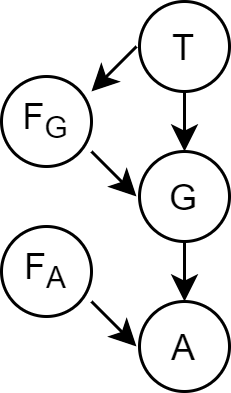
\includegraphics[scale=.5]{pics/Q14-13.png}
\end{figure}

\noindent 2) The network is not a polytree because there is a set of 3 nodes with connections between them, disallowing the label `tree'.\\

\noindent 3)
\begin{tabular}{|c||c|c|c|c|}
\hhline{-||----}
& \multicolumn{2}{c}{\textbf{F$_G$ True}} & \multicolumn{2}{|c|}{\textbf{F$_G$ False}}\\[-.2em]
\hhline{~::----}
 & \textbf{T High} & \textbf{T Normal} & \textbf{T High} & \textbf{T Normal}\\
\hhline{=::====}
G Normal & (1-y) & y & (1-x) & x \\
\hhline{-||----}
G High & y & (1-y) & x & (1-x) \\
\hhline{-||----}
\end{tabular}\\\\

\noindent 4)
\begin{tabular}{|c||c|c|c|c|}
\hhline{-||----}
& \multicolumn{2}{c}{\textbf{G Normal}} & \multicolumn{2}{|c|}{\textbf{G High}}\\[-.2em]
\hhline{~::----}
 & \textbf{F$_A$ True} & \textbf{F$_A$ False} & \textbf{F$_A$ True} & \textbf{F$_A$ False}\\
\hhline{=::====}
A On & 0 & 0 & 0 & 1 \\
\hhline{-||----}
A Off & 1 & 1 & 1 & 0 \\
\hhline{-||----}
\end{tabular}\\\\

\noindent 5) As alarm is only influenced by G, I will consider only G.\\\\
\indent $P(T_{High}|G,\neg F_G)$ = {\Large $\frac{P(G|T_{High},\neg F_G)P(\neg F_G|T)P(T)}{P(G,\neg F_G)}$}\\



\noindent \hrulefill \\\pagebreak



\centerline{- 14.18 - }
\ \\
\noindent 1) $P(B|j,m) = \alpha * P(B) *\sum_e P(e) *\sum_a P(a|b,e) P(j|a) P(m|a)$\\\\
\indent $\alpha * P(B) *\sum_e P(e) * \Big(0.9*0.7*\begin{pmatrix}0.95 & 0.94\\ 0.29 & 0.001\end{pmatrix} + 0.05*0.01*\begin{pmatrix}0.05 & 0.06\\ 0.71 & 0.999\end{pmatrix}\Big)$\\\\
\indent $\alpha * P(B) *\sum_e P(e) * \Big(0.63*\begin{pmatrix}0.95 & 0.94\\ 0.29 & 0.001\end{pmatrix} + 0.00005*\begin{pmatrix}0.05 & 0.06\\ 0.71 & 0.999\end{pmatrix}\Big)$\\\\
\indent $\alpha * P(B) *\sum_e P(e) * \Big(\begin{pmatrix}0.5985 & 0.5922\\ 0.1827 & 0.00063\end{pmatrix} + \begin{pmatrix}0.000025 & 0.00003\\ 0.000355 & 0.0005\end{pmatrix}\Big)$\\\\
\indent $\alpha * P(B) *\sum_e P(e) * \Big(\begin{pmatrix}0.598525 & 0.59223\\ 0.183055 & 0.00113\end{pmatrix}\Big)$\\\\
\indent $\alpha * P(B) *\Big(0.002 * \begin{pmatrix}0.598525 \\ 0.183055 \end{pmatrix}+0.998*\begin{pmatrix}0.59223 \\ 0.00113\end{pmatrix}\Big)$\\\\
\indent $\alpha * P(B) *\Big(\begin{pmatrix}0.001197 \\ 0.000366 \end{pmatrix}+\begin{pmatrix}0.591046 \\ 0.001128\end{pmatrix}\Big)$\\\\
\indent $\alpha * P(B) *\Big(\begin{pmatrix}0.592243 \\ 0.001493 \end{pmatrix}\Big)$\\\\
\indent $\alpha * (0.001 * 0.592243)(0.999 * 0.001493)$\\[0.4em]
\indent $\alpha * (0.000592)(0.001492)$\\[0.4em]
\indent $\langle0.28428, 0.71616\rangle$\\[0.4em]


\noindent 2) \# Additions = 6\\
\indent \# Multiplications = 16\\
\indent \# Divisions = 2\\
\indent Total = 24\\[.4em]
\indent The algorithm will perform 27 operations.\\\\


\noindent 3) Enumeration requires parsing through 2 complete binary trees for each variable, \\
\indent each one with a depth of n-2. This leaves computation at O(2$^n$).\\
\indent Elimination only considers 2 variables at a time, working through each variable one\\
\indent at a time. Thus, the algorithm runs for all n variables at O(n).\\




\end{document}

















